\section{Vehicle description}
The track vehicle provided for the project can be seen on \figref{TrackedVehicle} in \secref{PrototypeConstraints}. A platform of the same size of the vehicle  is mounted on the vehicle, to protect the servo and the mechanical system and to support the system, which include PCB boards, the battery, and the sensors used to control the path of the vehicle. When the platform is mounted on, the vehicle is 45 cm long, 29 cm in width, 12 cm in height and it weighs 2932 grams.
The following sections will analyse the vehicle mechanical system and the features that the vehicle use to drive and steer.

\subsection{Drivetrain}

The drivetrain of a motor vehicle, is the components, that transfer the rotanial energy from the motor to the driving wheel of the vehicle. For this vehicle, the drivetrain will contains the gear connected to the motor, the differential gear box and the gears connected to the belts. The drivetrain is shown on \figref{vehicleDescriptionDriveTrain}.

\begin{figure}[H]
	\centering
	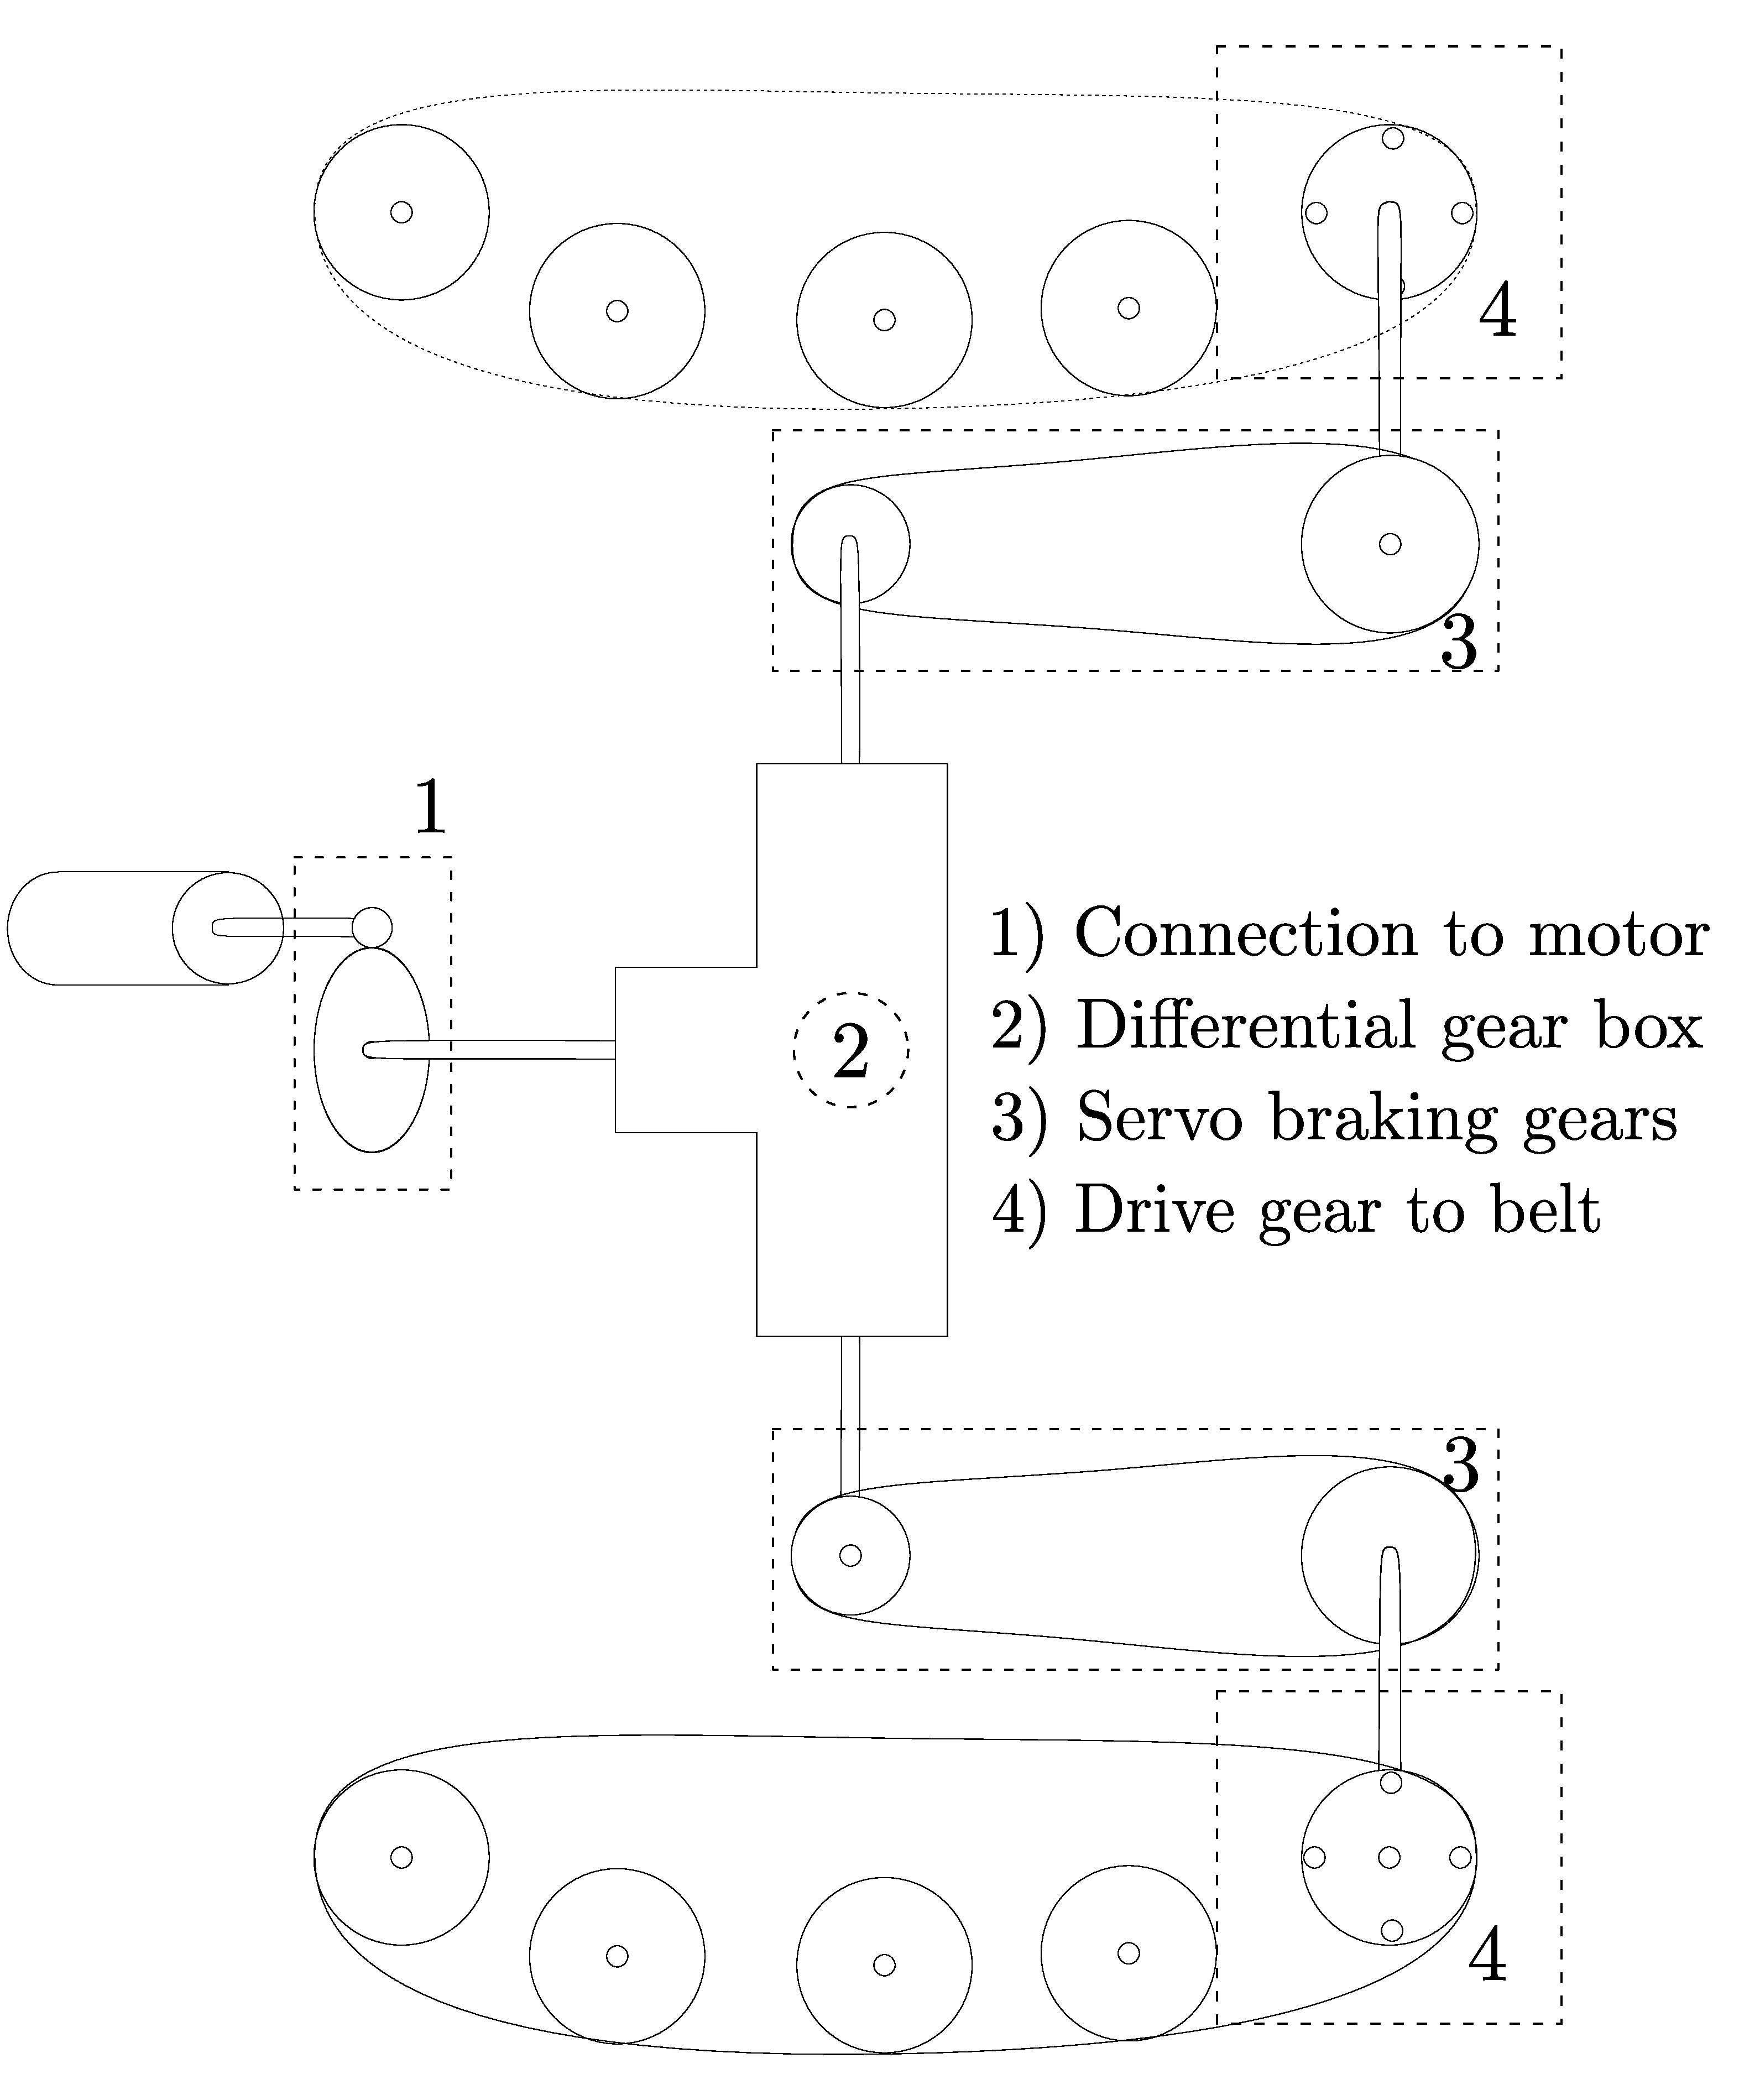
\includegraphics[scale=0.2]{figures/vehicleDescriptionDriveTrain.pdf}
	\caption{Illustration of the drive train of the vehicle.}
	\label{vehicleDescriptionDriveTrain}
\end{figure}

The vehicle is composed of two tracks enveloping 4 wheels, plus a gear connected to the differential gear box. The servomotor in (3) controls the steering of the vehicle by braking one track or another, so that the main motor only control the absolute speed and not the turning. The differential gear, in (2), is powered direcly by the motor.\\
A Hall sensor, in (4), is plugged on each gear wheel to control the speed of each belt.\\
 This section will describe more accurately different part of the vehicle seen in this picture.\\